\section{Methods}
\label{sec:methods}

\indent We needed to accurately detect keypoints to extract poses and gestures from, and to do this we needed a model that could help us achieve that. 

\subsection{Keypoint Detection with OpenPose}
\indent We had three main criteria when selecting an existing library with which to detect body parts.
\begin{enumerate}
    \item The library had to store model outputs in an easily readable, non-proprietary format, such as JSON, 
    so that we could easily work with it.
    \item The model must perform reasonably well on a CPU. When we began our project, we were unsure of how 
    to secure GPU access, and we needed a model that could provide meaningful outputs even if we failed to 
    set up a system for using GPUs.
    \item Ideally, the model possessed capability to detect multiple people in a given frame. Although we did 
    not prioritize our product’s ability to process videos with multiple people, we wanted the flexibility to 
    add that functionality later without a potential overhead from switching our library of choice.
\end{enumerate}
\indent With the above considerations in mind, we evaluated MediaPipe, MoveNet, and OpenPose.

\indent We first explored MediaPipe, a versatile framework by Google that supported vision, natural language, and audio 
tasks. With its lightweight design for on-device ML and target towards time-series data, we found its performance 
promising. However, it appeared to only support single-person pose detection, so we set it aside early on to 
spare our future selves the pain of transitioning to a different library.
	
\indent We also investigated Tensorflow’s MoveNet, incidentally also part of Google. Built upon MobileNet, it had a 
satisfyingly low resource consumption. However, with the initial configurations that we had tested, it seemed to 
have poor accuracy, with keypoints often hovering in the general region of the desired body parts, but not truly 
aligning with the body joints. Because physical therapy patients may have injuries that cause lower tolerances 
for certain movements, we decided against using MoveNet.
	
\indent Finally, we decided to try OpenPose. We quickly learned of its ability to output key points from each frame of a 
video as a JSON file. Additionally, not only does OpenPose enable multi-person pose detection, but it also appeared 
to support 3D keypoint detection when two camera perspectives were provided. While we did not plan for the possibility 
of 3D keypoint detection, we were intrigued by the potential, and believed its progress to be evidence that OpenPose 
was still being maintained. Hence, we chose OpenPose for keypoint detection.
	
\indent While OpenPose does have a higher performance overhead than the other two models, we consider it a worthy trade for the 
improved accuracy and the increased options for input videos (many of which may have more than one person). In fact, while 
testing OpenPose’s hyperparameters, we learned that lowering the video resolution caused a significant speedup in 
processing time, but we were ultimately against reducing the resolution in our input videos because our project 
performance doesn’t depend on low latency, but it does benefit from higher accuracy.

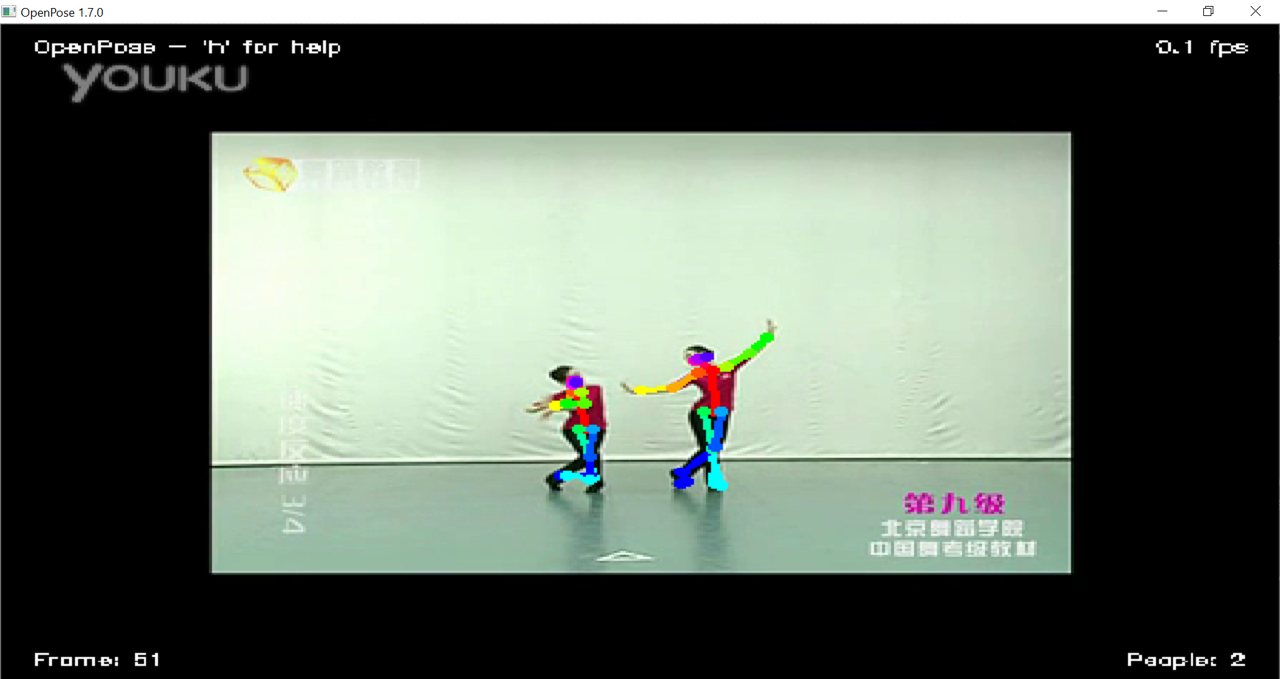
\includegraphics[width=\columnwidth]{sec/openpose_demo}
\textit{Figure 1. OpenPose in action: pose detection on a frame from an input video of two people. 
OpenPose accurately detects the key points on both people despite their slightly unorthodox body positions.}

\subsection{Feature Transform}
\indent For a given video, OpenPose outputs a directory of JSON files, with one for each frame. Before passing these outputs to a 
second machine learning model, we wanted an algorithm that could map similar poses and movements to the same values, 
regardless of camera angle or relative location of the person to the camera. (Due to the nature of OpenPose outputting x, 
y values for keypoints, we have already circumvented the issue of changes in illumination.)  Our keypoint-to-angle algorithm 
aims to:
\begin{enumerate}
    \item Greatly reduce the role of absolute pixel locations in identifying features
    \item Make the model invariant to differences in the user’s body structure
    \item Detect straight-line, elliptical, and hybrid motion
\end{enumerate}

\indent We choose to transition away from absolute positions due to inspiration from SIFT’s usage of illumination gradients over 
absolute color values. Absolute positions could cause our model to unintentionally train on an individual's location in the 
camera view. Similarly, we hoped to make our model invariant to the user’s height and distance from the camera 
(people in the foreground tend to appear taller than people in the background). 

\indent Thus, we decided to add some math equations to transform our features from absolute x, y positions to angles between detected 
key points. Additionally, this will likely aid the model in recognizing elliptical motions, which are prevalent in physical 
therapy exercises, as a continuous motion, as opposed to a given, singular elliptical motion being calculated as multiple 
straight-line movements. Additionally, this encodes information about body parts relative to each other. For 
instance, moving one’s right hand downwards on the left side of one’s body could be differentiated from moving 
one’s right hand downwards on the right side of one’s body through the angle of the right elbow relative to 
the right shoulder.

\subsection{Pose and Gesture Extraction}
\indent By the temporal nature of videos and humans’ inability to teleport, many frames have body angles that are 
close in value to those of the neighboring frames, similar to how in images, many pixels may have color 
values close to their neighbors. It would be inefficient to always work with all of the frames in a given 
video. In fact, in images, features are often only extracted for corners. We suggest the idea of extracting 
poses and gestures from videos.

\indent While the algorithm we’ve designed is inspired by the Harris Corner Detector, poses and gestures differ from 
corners in that we’re not looking for a gradient across all dimensions. Intuitively, this makes sense: even 
if a person were to stand in place (not change the angles in their lower body), we would still consider a 
hand-wave to be a gesture, and raising different hands would be considered different poses. 

\indent To reiterate, unlike a corner, which only has two dimensions x and y, a pose or gesture would have as many 
dimensions as there are angles. Additionally, while corners are detected based on the ratio of the 
eigenvalues, we’re more concerned with having one strong edge or many weak edges in identifying a gesture: 
requiring all angles to change would omit basic gestures like a simple hand wave because the majority of 
angles in the body wouldn’t change. Hence, we use Euclidean Distance as a “change in body position” score.

\indent Another point of interest is that poses would have a low “change in body position” score. Going back to the 
corner detection analogy, poses are analogous to a flat area within an  image, yet they arguably define a 
person’s physical actions more than the brief moments of highest “change in body position.” Thus, to extract 
poses from angles, we actually apply non-minimum suppression (instead of the Harris Corner Detector’s 
non-maximum suppression) after calculating the Euclidean Distance between angles in adjacent frames.

\indent Meanwhile, we consider a gesture to be the opposite of a pose, a small range of frames when there is a 
significant “change in body position.” Arguably, a gesture would take place for all the frames between 
two poses, not just for moments of the fastest “change in body position.” However, because we applied a 
threshold that selects only a subset of the most significant poses, the above definition may cause multiple 
gestures to be recognized as one, so we have currently defined a gesture to be three consecutive frames of 
significant change in angles. (However, it could be interesting to explore modified algorithms for detecting 
poses and gestures in future work.)

\subsection{Distance Evaluation}
\indent Our project uses three versions of Euclidean Distances for 
various functions: 1) the default formula identifies poses and gestures 
and suppress the non-maximum/minimum cases, 2) the formula on a subset 
of columns to calculate a quantitative score to show the user their 
similarity to the physical therapy video, and 3) a modified combination 
of floored angle gradients and weighted Euclidean Distance. 

\subsection{Video Selection}
\indent To test our model, we first selected videos from Cornell 
University’s CornellHealth website\cite{Alpher11}. These are legitimate 
physical therapy videos that get prescribed to current patients by their 
Cornell Health physical therapist, making them an ideal dataset to base 
our pose estimation model on.

\indent We then completed these exercises ourselves to obtain a sample 
set of testing videos. We were able to compare the instructional videos 
with the videos of ourselves following the exercises. The accuracy of 
our model was determined by comparing our test video with the Cornell 
video, and determining on our own if the numerical accuracy generated 
by the model seemed accurate. For example, a patient video following 
the instructional video perfectly should yield a 100\% accuracy score, 
whereas a patient video that does not follow the instructional video 
well should yield a lower score.
